\documentclass{exam}
\usepackage{main}
\author{}
\title{Evaluation de cours}
\date{18 Décembre 2023}

\qformatExos
\begin{document}
\maketitle
\begin{questions}
\question Soit deux fonctions $f$ et $g$ définies sur $[-3;5]$ dont les courbes représentatives sont données ici.
\begin{center}
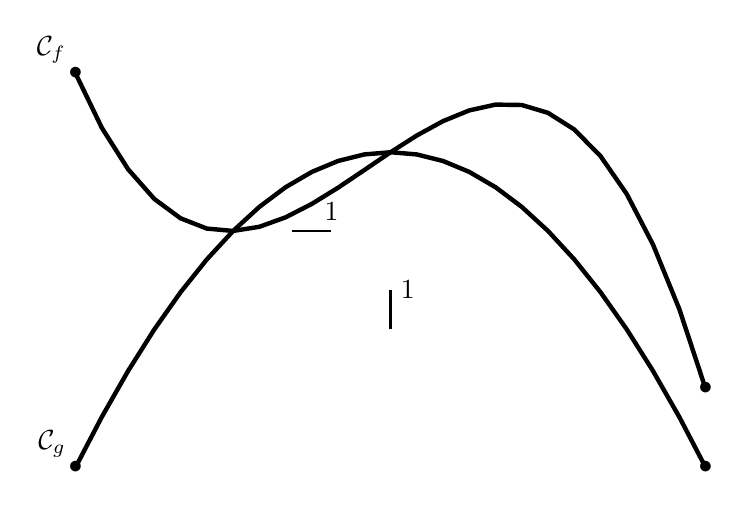
\begin{tikzpicture}
\shorthandoff{:};
\millirepere[step=1](-3.5,-4.5) -- (5.5,4.5);
\draw[domain=-3:5, ultra thick] plot (\x,{-(\x*\x)/4 + \x/2 + 7/4});
\draw[domain=-3:5, ultra thick] plot (\x,{-(7*\x*\x*\x)/96 + 5*\x*\x/32 + 55*\x/96 + 43/32});
\draw[thick] (1,-0.25) -- (1,0.25) node[right] {$1$}; 
\draw[thick] (-0.25,1) -- (0.25,1) node[above] {$1$};
\draw (-3,3) node {$\bullet$} node[above left] {$\mathcal{C}_f$};
\draw (-3,-2) node {$\bullet$} node[above left] {$\mathcal{C}_g$};
\draw (5,-1) node {$\bullet$};
\draw (5,-2) node {$\bullet$};
\end{tikzpicture}    
\end{center}
\begin{parts}
\part Résoudre $f(x) = g(x)$.
\part Résoudre $g(x) < f(x)$.    
\end{parts}
\end{questions}
\end{document}